\documentclass{article}

\usepackage[top=0.5in, bottom=0.8in, left=0.5in, right=0.5in]{geometry}

\widowpenalty10000
\clubpenalty10000

\usepackage{tgheros}
\renewcommand*\familydefault{\sfdefault}
\usepackage[T1]{fontenc}

\usepackage{tabularx}
\def\arraystretch{1.4}

\usepackage{multicol}
\usepackage{multirow}
\usepackage{hhline}
\setlength\columnsep{2em}

\usepackage{titlesec}
\newcommand{\sectionbreak}{\clearpage}

\usepackage{graphicx}
\graphicspath{ {images/} }

\usepackage{xcolor}
\definecolor{lightBlue}{rgb}{0.8,0.9,1.0}

\setlength{\parindent}{0pt}
\setlength{\parskip}{0pt}

\usepackage{enumitem}
\setitemize{itemsep=3pt, topsep=1.5ex, parsep=0pt, partopsep=0pt}
\setenumerate{itemsep=3pt, topsep=1.5ex, parsep=0pt, partopsep=0pt}

\setlist[itemize]{leftmargin=1.5ex}

\renewcommand\labelitemi{$\vcenter{\hbox{\tiny$\bullet$}}$}

\usepackage{numprint}
\npthousandsep{,}

\newcommand\TV{1500}
\newcommand\TVsevens{1000}
\newcommand\TVdivisor{1000}
\newcommand\TVGP{\the\numexpr\TV*\TVdivisor\relax}

% set up one line title
\makeatletter
\renewcommand\@maketitle{%
{\LARGE \@title }
}
\makeatother

\title{Basic Blood Bowl}
\date{2017-07-31}
\author{ibsh}

\begin{document}

\raggedcolumns

% display one line title
\maketitle
\thispagestyle{empty}

\begin{multicols}{2}

\section{Game rules}

\subsection{Setting up the game}
\par Lay out the board and gather the players, dice and templates. Each coach will need their team, a dugout and a set of counters.
\par Each coach should place a Turn counter, a Score counter, and a Re-roll counter on the appropriate tracks.
\par Flip a coin; the winner chooses whether to kick or receive.

\begin{itemize}
\item The kicking team always sets up first.
\item A team must field eleven players and no more. If fewer than eleven players are available, field as many as you can.
\item At least three players must be set up next to the half way line, on the Line of Scrimmage. If fewer than three players are available you concede the match.
\item No more than two players may be set up in each wide zone.
\end{itemize}

\subsection{The kick-off}
\par After both teams have set up, the coach of the kicking team places the ball in any square in the opponent's half of the pitch (including the End Zone). Kicks are very inaccurate, so scatter the ball (D6 squares in a direction determined by D8) to determine where it will land. Before the ball lands, roll on the kick-off table:

\medskip
\begin{tabularx}{\linewidth}{ | c | X | }
\hline
\textbf{2D6} & \textbf{Kick-Off Event} \\ 
\hline
2 & \textbf{Get the ref}: no players may be sent off for fouling during this drive. \\
\hline
3 & \textbf{Riot}: if this kick-off precedes the first turn of the half for the receiving team, move both teams' turn markers forward one space; if the last turn, move them both backward one space. Prior to any other turn, flip a coin to determine which direction to move them. \\
\hline
4 & \textbf{Instinctive defence}: the coach of the kicking team may set the team up again, though the new setup must remain legal. The receiving team must remain in their existing positions. \\
\hline
5 & \textbf{High kick}: any one player on the receiving team who is not in an opposing player's tackle zone may be moved into the square where the ball will land, as long as the square is unoccupied, regardless of their MA. \\
\hline
6 & \textbf{Cheering fans}: each coach rolls a D3; the side with the highest score gets an extra re-roll this half. In case of a tie, both teams get an extra re-roll. \\
\hline
7 & No special event. \\
\hline
\end{tabularx}

\begin{tabularx}{\linewidth}{ | c | X | }
\hline
8 & \textbf{Brilliant coaching}: each coach rolls a D3; the side with the highest score gets an extra re-roll this half. In case of a tie, both teams get an extra re-roll. \\
\hline
9 & \textbf{Quick Snap}: the offence start their drive a moment before the defence is ready; all of the players on the receiving team may move one square. This is a free move and may be made, ignoring tackle zones, into any adjacent empty square, including on the opposing half of the pitch. \\
\hline
10 & \textbf{Blitz}: the defence start their drive a moment before the offence is ready; the kicking team receives a free bonus turn, although any players starting in an enemy tackle zone may not perform an action. Rules for team re-rolls and turnovers apply as usual. \\
\hline
11 & \textbf{Throw a rock}: Each coach rolls 2D6; the high scorer's fans throw a rock at an opposing player. A tie means that both teams are affected. Select a player on the affected team(s) at random (only players on the field are eligible) and place them Stunned. \\
\hline
12 & \textbf{Pitch invasion}: Each coach rolls a D6 for each opposing player on the pitch; if the roll is a 6, place the player Stunned. \\
\hline
\end{tabularx}
\medskip

\par After the kick-off table takes effect, the ball lands:
\begin{itemize}
\item If it lands in an empty square it will bounce one more square.
\item If it lands on a square occupied by a player, they must try to catch the ball.
\item If it scatters or bounces off the pitch, or into the kicking team's half, the receiving coach is awarded a Touchback and must give the ball to any player on their team. 
\end{itemize}
\par Once the kick-off has been taken you are ready to proceed to the first turn of the game.

\subsection{The sequence of play}
\par Blood Bowl is split into two halves of sixteen turns each (i.e. eight turns per coach). The game is played using a simple but strict sequence of play, with the receiving team taking a turn, followed by the kicking team, one after the other, until the end of the drive. A drive is defined as playing until a touchdown is scored or the half ends.

\subsection{Taking a turn}
\par Move the Turn counter one space along its track, then perform one Action with each player on the team.

\subsection{Player actions}
\par Each player on a team may perform one Action per turn.
\par You must declare which Action a player is going to take before carrying it out.
\par Players perform Actions one at a time. A player must finish their Action before another player can take one.
\par Actions other than Move and Block may only be declared once per turn.

\medskip
\begin{tabularx}{\linewidth}{ | X | }
\hline
\textbf{Move}: The player may move a number of squares equal to their MA. \\
\hline
\textbf{Block}: The player may make a single block against a player in an adjacent square. \\
\hline
\textbf{Blitz}: The player may move a number of squares equal to their MA. They may make one block at any point during the move, which costs one square of movement. \\
\hline
\textbf{Pass}: The player may move a number of squares equal to their MA. At the end of the move the player may pass the ball. \\
\hline
\textbf{Hand-off}: The player may move a number of squares equal to their MA. At the end of the move the player may hand off the ball. \\
\hline
\textbf{Foul}: The player may move a number of squares equal to their MA. At the end of the move the player may foul a Prone or Stunned opponent. \\
\hline
\end{tabularx}
\medskip

\subsection{Turnovers}
\par Normally, a turn ends when all of the players on the team have performed an Action, or the coach decides not to take any more Actions. However, certain events, called turnovers, cause a turn to end early:

\begin{itemize}
\item A player on the moving team is Knocked Down (though being injured by the crowd or being placed Prone is not a turnover unless the player is holding the ball)
\item A passed ball, or hand-off, is not caught by a member of the moving team before the ball comes to rest
\item A player from the moving team attempts to pick up the ball and fails
\item A pass attempt is fumbled (even if a player from that team catches the fumbled ball)
\item A player is ejected by the referee for a foul
\item A player attempts to throw a team-mate holding the ball and the ball carrier fails to land successfully (including due to a failed Always Hungry roll)
\end{itemize}

\par A coach that suffers a turnover is not allowed to take any further actions that turn, and any action being taken ends immediately even if it was only partially completed. Make armour and injury rolls for players that were knocked down, and if the ball was dropped then roll to see where it bounces to. Players who were stunned on previous turns should be turned face up, and then the opposing coach may start to take their turn.

\subsection{The Agility table}
\par The Agility table is used to work out the success or failure of a number of different Actions in Blood Bowl, including dodging, picking up the ball, and throwing or catching the ball. Each Action has its own set of modifiers.
\par A roll of 1 before modification always fails and a roll of 6 before modification always succeeds, for any Agility roll made during a game.

\medskip
\begingroup\setlength{\fboxsep}{0pt}\colorbox{lightBlue}{%
\begin{tabularx}{\linewidth}{ | X | c | c | c | c | c | c | }
\hline
\multicolumn{7}{| l |}{\textbf{Agility Table}} \\
\hline
AG & 1 & 2 & 3 & 4 & 5 & 6+ \\
\hline
Required D6 roll & 6+ & 5+ & 4+ & 3+ & 2+ & 1+ \\
\hline
\end{tabularx}%
}\endgroup
\medskip

\subsection{Movement}
\par A player may move a number of squares less than or equal to their Movement Allowance. Players may move in any direction or combination of directions, including diagonally, as long as they do not enter a square that holds another player.

\subsection{Tackle zones}
\par A standing player exerts individual tackle zones on each of the eight adjacent squares. A player who is Prone or Stunned does not exert any tackle zones.
\par In order to leave a square that is in one or more opposing tackle zones, a player must dodge. The player only has to dodge once in order to leave the square, no matter how many opposing tackles zones are on it.

\medskip
\begingroup\setlength{\fboxsep}{0pt}\colorbox{lightBlue}{%
\begin{tabularx}{\linewidth}{ | X | c | }
\hline
\multicolumn{2}{| l |}{\textbf{Dodge modifiers}} \\
\hline
Making a Dodge roll & +1 \\
\hline
Per opposing tackle zone on the square the player is dodging to & -1 \\
\hline
\end{tabularx}%
}\endgroup
\medskip

\par Make an agility roll with the appropriate modifiers for dodging. If it succeeds, the player may carry on moving (and dodging if required) until they have used up their full Movement Allowance. If it fails, the player is Knocked Down in the square they were dodging to (a roll must be made to see if they were injured) and the team suffers a turnover, ending their turn immediately.

\subsection{Going for it}
\par When a player takes any Action that involves moving, they may try to move one or two extra squares over and above their MA -- this is called "going for it".
\par Roll a D6 for the player after they have moved each extra square. On a roll of 1 the player trips and is Knocked Down in the square that they moved to; the opposing coach must roll to see if the player was injured. On any other roll the player moves without mishap. If the player is Knocked Down then their team suffers a turnover and their turn ends immediately.
\par A player that is taking a Blitz Action may "go for it" in order to make a block. Roll a D6 for the player after declaring that they will make the block. On a roll of 1 the player is Knocked Down as described above. On any other roll the player makes the block without mishap.

\subsection{Picking up the ball}
\par If a player moves into a square in which the ball is lying, they must attempt to pick it up. Players that move into the square with the ball at other times cannot pick up the ball, and instead it will bounce one square; this does not cause a turnover.

\medskip
\begingroup\setlength{\fboxsep}{0pt}\colorbox{lightBlue}{%
\begin{tabularx}{\linewidth}{ | X | c | }
\hline
\multicolumn{2}{| l |}{\textbf{Pick up modifiers}} \\
\hline
Picking up the ball & +1 \\
\hline
Per opposing tackle zone on the player & -1 \\
\hline
\end{tabularx}%
}\endgroup
\medskip

\par Make an agility roll with the modifiers for picking up the ball. If it succeeds, the player picks up the ball (place it on their base) and may carry on with their turn. If the roll fails, the player drops the ball, which will bounce one square; their team suffers a turnover and their turn ends immediately.

\subsection{Blocks}
\par Instead of moving, a player may throw a block at an opposing player in an adjacent square.  Players that are Prone may not perform a block,  and you may only make a block against a standing player. To see if a block works you will need to use the special Block dice.

\subsubsection{Blitzes}
\par Once per turn a player on the moving team is allowed to make a special Blitz move; the player may move and make a block. The block may be made at any point during the move, but costs one square of movement. The player may carry on moving after the effects of the block have been worked out, if they have any squares of movement left.

\subsubsection{Strength}
\par The number of dice that are rolled depends on the strengths of the two players involved. Obviously, if one player is stronger than the other they are more likely to knock down their opponent when they make a block:

\begin{itemize}
\item If the players' strengths are equal, one dice is rolled.
\item If one player is stronger, two dice are rolled and the stronger player may choose which one is used.
\item If one player is more than twice as strong, three dice are rolled and the stronger player may choose which is used.
\end{itemize}

\par Note that the coach of the player making the block always rolls the dice, but that the coach of the stronger player chooses which is used.

\subsubsection{Assisting a block}
\par After a block has been declared, team-mates of the attacker and the defender may give an assist. This allows two or more attackers to gang up on a single defender, or for one or more defenders to aid a companion against a block. Each of these extra players adds +1 to the Strength of the player that they are assisting. Assisting a block does not count as an Action, and a player can assist any number of blocks per turn. A player is allowed to make an assist even if they have moved or taken an Action.
\par The attacking coach must declare if any of their players will give an assist first, then the defending coach must add defensive assists with players from their team. In order to make an assist, the player:

\begin{itemize}
\item must be adjacent to the enemy player involved in the block.
\item must not be in the tackle zone of any other player from the opposing team.
\item must be standing.
\item must have their tackle zones.
\end{itemize}

\par The result of the block only affects the two players directly involved; any assisting players are not affected. Similarly, only the skills belonging to the two players directly involved in the block may be used on the result; skills belonging to assisting players cannot be taken advantage of by either side.

\subsubsection{Rolling the block dice}
\par To complete the block action, roll the appropriate number of dice and look up the result below:

\medskip

\begin{tabularx}{\linewidth}{  c  X  }
\raisebox{-.6\height}{
\includegraphics[width=3em]{ad}} & \textbf{Attacker Down}: The attacking player is Knocked Down. \\
\raisebox{-.6\height}{
\includegraphics[width=3em]{bd}} & \textbf{Both Down}: Both players are Knocked Down in their current squares, unless one or both of the players involved uses the Block skill; if a player uses the Block skill then they are not Knocked Down. \\
\raisebox{-.6\height}{
\includegraphics[width=3em]{pb}} & \textbf{Pushed Back}: The defending player is pushed back one square by the blocking player. The attacking player may follow up the defender. \\
\raisebox{-.6\height}{
\includegraphics[width=3em]{ds}} & \textbf{Defender Stumbles}: Unless the defender uses the Dodge skill they are pushed back and then Knocked Down. If they use the Dodge skill then they are only pushed back. The attacking player may follow up the defender. \\
\raisebox{-.6\height}{
\includegraphics[width=3em]{dd}} & \textbf{Defender Down}: The defending player is pushed back and then Knocked Down. The attacking player may follow up the defender. \\
\end{tabularx}
\medskip

\subsubsection{Push backs}
\par A player that is pushed back as a result of a block must be moved one square away from the player making the block; there are three eligible squares in each direction:
\medskip
\begin{center}
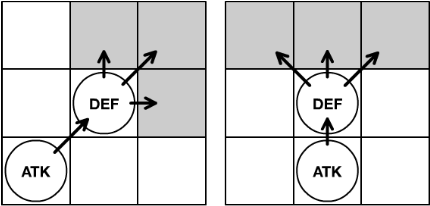
\includegraphics[width=0.6\columnwidth]{pushbacks}
\end{center}
\par The coach of the player who made the block may decide which square the player is moved to. The player must be pushed back into an empty square if possible. A square containing only the ball is considered empty, and a player pushed to it will cause the ball to bounce. If all such squares are occupied by other players, then the player is pushed into an occupied square, and the player that originally occupied the square is pushed back in turn. This secondary push back is treated exactly like a normal push back (Prone and Stunned players may be pushed in this manner as well). The coach of the moving team decides all push back directions for secondary push backs, unless the pushed player has a skill that overrides this.
\par Players must be pushed off the pitch if there are no eligible empty squares on the pitch. A player pushed off the pitch, even if Knocked Down, is beaten up only by the crowd and receives a roll on the Injury Table. The crowd does not have any injury modifying skills. Note that no Armour roll is made for a player that is pushed off the pitch: they are automatically injured. If a Stunned result is rolled on the Injury table the player should be placed in the Reserves box of the Dugout, and must remain there until the end of the drive. If the player who is holding the ball is pushed out of bounds, then they are beaten up by the fans, who are more than happy to throw the ball back into play! The throw-in template is centred on the last square the player was in before they were pushed off the pitch.

\subsubsection{Following up}
\par A player who has made a block is allowed to make a special follow up move and occupy the square vacated by the player that they have pushed back. The player's coach must decide whether to follow up before any other dice rolls are made. This move is free, and the player can ignore enemy tackle zones when they make the move (they do not have to dodge to enter the square). Players that are blitzing are allowed to make follow up moves, and the move does not cost them any more of their movement (they already paid a square in order to make the block).

\subsubsection{Knock downs}
\par A player that is Knocked Down should be placed on their side in the square, face up. The player may be injured. If the player who is Knocked Down comes from the moving team, this causes a turnover and the moving team's turn ends immediately.
\par Players that are Knocked Down or placed Prone for any reason should be placed face up on the pitch in the square they were in when they fell over. While Prone, the player loses their tackle zones and may do nothing until they stand up when they next take an Action.
\par A player who is carrying the ball and who is knocked down or placed Prone will drop the ball in the square where they fall. The dropped ball will bounce one square in a random direction after the player's armour/injury rolls are fully resolved.

\subsubsection{Injuries}
\par Unless the rules state otherwise, any player that is Knocked Down may be injured. The opposing coach rolls 2D6 in an attempt to beat the Knocked Down player's Armour value. If the roll succeeds, they roll on the Injury table to see what injury the player has suffered:

\medskip
\begin{tabularx}{\linewidth}{ | c | X | }
\hline
\textbf{2D6} & \textbf{Injury} \\
\hline
2-7 & Stunned: Leave the player on the pitch, but turn them face-down. All face-down players are turned face up at the end of their team's next turn (not the turn they are stunned), even if a turnover takes place. Once face-up they may stand up on any subsequent turn using the normal rules. Stunned players recover automatically at the end of the drive. \\
\hline
8-9 & KO: Take the player off the pitch and place them in the Dugout in the KO box. They will have a chance to recover at subsequent kick-offs. \\
\hline
10-12 & Casualty: Take the player off the pitch; they must miss the rest of the match. The opposing coach must roll on the casualty table to see if the player suffers any long-term effects. \\
\hline
\end{tabularx}
\medskip

\medskip
\begin{tabularx}{\linewidth}{ | c | X | }
\hline
\textbf{D6} & \textbf{Casualty} \\
\hline
1-3 & Badly Hurt: No long-term effect. \\
\hline
4 & Nasty Injury: Miss the next game. \\
\hline
5 & Niggling Injury: Miss the next game. Subsequent injury rolls against this player gain +1 per Niggling Injury. \\
\hline
6 & Dead \\
\hline
\end{tabularx}
\medskip

\par The coach of a player that suffers a casualty should make a note of its effect on their team roster.

\subsubsection{Substitutes}
\par You may not substitute fit players for injured players or players that have been sent off while a drive is in progress. The only time that you may add reserves is when you are setting up after a touchdown has been scored, or when setting up after half time.

\subsubsection{Standing up}
\par The only time a player can stand up is at the beginning of an Action, at a cost of three squares from their movement. If the player has fewer than three squares of movement, they must roll 4+ to stand up: if they stand up successfully, they may not move further squares unless they Go For It. Failure to stand successfully does not cause a turnover.
\par Players may stand up in an opposing player's tackle zone without having to make a Dodge roll. Note that a player who stands up may not take a Block Action.

\subsection{Passing}
\par Once per turn a player on the moving team is allowed to make a Pass Action. The player is allowed to make a normal move, and after they have completed the move they may throw the ball. Note that the player does not have to be holding the ball at the start of the Action; they could use their move to run over and pick up a ball on the ground and then throw it, for example.
\par Declare a Pass Action, move if desired, and then start the throw. It is perfectly acceptable to pre-measure the range to several players at any point during the throwing player's move before you declare the target of the pass. Once you have thrown the ball, you may not move the throwing player any farther that turn.

\begin{enumerate}
\item Declare the target of the pass and determine the appropriate range modifier.
\item Roll for any eligible interception.
\item Make an agility roll for the pass. If the pass is fumbled, suffer a turnover.
\item If the pass is inaccurate, scatter 3 times (to represent where the inaccurate pass lands, not the ball bouncing).
\item If the ball lands in a square with a player, roll to catch, otherwise bounce the ball once from the empty square the ball landed in.
\end{enumerate}

\subsubsection{Interceptions}
\par One player on the opposing team may attempt to intercept a thrown ball. Only one player can attempt an interception, no matter how many are eligible. To be able to make an interception, the player must:

\begin{itemize}
\item have the plastic ruler pass over at least part of the square they are standing in.
\item be closer to the thrower than the target square is.
\item be closer to the target square than the thrower is.
\item have their tackle zones.
\item The coach must declare that one of their players will try to intercept before the thrower rolls to see if they are on target.
\end{itemize}

\par Make an Agility roll with the modifiers for Interception.

\medskip
\begingroup\setlength{\fboxsep}{0pt}\colorbox{lightBlue}{%
\begin{tabularx}{\linewidth}{ | X | c | }
\hline
\multicolumn{2}{| l |}{\textbf{Interception modifiers}} \\
\hline
Attempting an interception & -2 \\
\hline
Per opposing tackle zone on the player & -1 \\
\hline
\end{tabularx}%
}\endgroup
\medskip

\par If it fails, the pass carries on as normal. If it succeeds, the player has caught the ball (place it on the player's base). A successful interception causes a turnover, and the moving team's turn ends immediately.

\subsubsection{The throw}

\medskip
\begingroup\setlength{\fboxsep}{0pt}\colorbox{lightBlue}{%
\begin{tabularx}{\linewidth}{ | X | c | }
\hline
\multicolumn{2}{| l |}{\textbf{Passing modifiers}} \\
\hline
Throwing a Quick Pass & +1 \\
\hline
Throwing a Short Pass & +0 \\
\hline
Throwing a Long Pass & -1 \\
\hline
Throwing a Long Bomb & -2 \\
\hline
Per opposing tackle zone on the player & -1 \\
\hline
\end{tabularx}%
}\endgroup
\medskip

\par Make an Agility roll with the modifiers for passing. If the roll for a pass is 1 or less before or after modification, the thrower has fumbled and dropped the ball. The ball bounces once from the thrower's square, and the moving team suffers a turnover and their turn ends immediately.
\par If the pass is not fumbled but the roll fails, the pass is inaccurate and scatters 3 times before landing. If the roll succeeds, the pass is accurate and lands in the target square.

\subsubsection{Catching the ball}
\par If the ball lands in a square occupied by a standing player on either team, then they must attempt to catch the ball. Prone and Stunned players may never attempt to catch the ball.

\medskip
\begingroup\setlength{\fboxsep}{0pt}\colorbox{lightBlue}{%
\begin{tabularx}{\linewidth}{ | X | c | }
\hline
\multicolumn{2}{| l |}{\textbf{Catching modifiers}} \\
\hline
Catching an accurate pass or hand-off & +1 \\
\hline
Catching a missed pass, kick-off, bouncing ball or throw-in & +0 \\
\hline
Per opposing tackle zone on the player & -1 \\
\hline
\end{tabularx}%
}\endgroup
\medskip

\par Make an Agility roll with the modifiers for catching. If the roll succeeds, the player has caught the ball (place it on the player's base). If it fails, then the player drops the ball, which will bounce.

\subsubsection{Bouncing balls}
\par The ball bounces if:

\begin{itemize}
\item it is dropped or not caught.
\item it lands on or bounces to a square with a Prone or Stunned player.
\item a player is pushed to or lands in its square.
\item it lands in an unoccupied square.
\end{itemize}

\par To find out where the ball bounces to, roll for scatter. If the ball bounces into an occupied square, then the player in the square must attempt to catch it. If it bounces into an empty square, it stops. If it bounces off the field, a Throw-in occurs.

\subsubsection{Throw-ins}
\par When a ball scatters or bounces off the pitch it is immediately thrown back in by the spectators. Use the Throw-in template to work out where the ball goes, using the last square the ball crossed before going off as a starting point. The ball is thrown 2D6 squares in a direction determined by D3. Throw-ins cannot be intercepted.

\subsubsection{Turnovers}
\par If a pass isn't caught by a player from the moving team, this causes a turnover and the moving team's turn ends. The turnover does not take place until the ball finally comes to rest. This means that if the ball misses the target but is still caught by a player from the moving team, then a turnover does not take place. The ball could even scatter or bounce out of bounds, be thrown back into an empty square, and as long as it is caught by a player from the moving team then the turnover is avoided.

\subsection{Handing off the ball}
\par A hand-off is where the ball is simply handed to another player, friend or foe, in an adjacent square. No dice roll is required to see if the player attempting the hand-off is successful -- it automatically hits the targeted player. However, the player that the ball is handed off to must roll to see if they catch the ball, treating it as an accurate pass.

\subsection{Fouls}
\par Normally, players that are Prone or Stunned cannot be attacked. However, one player per turn is allowed to take a Foul Action. This allows the player to move a number of squares equal to their MA and then make a foul against an opposing player who is Prone or Stunned and in an adjacent square.
\par The coach nominates the victim, and then makes an Armour roll for them.

\begin{itemize}
\item Any of the fouler's teammates that are adjacent to the victim must assist, each extra player adding 1 to the Armour roll.
\item Any of the victim's teammates that are adjacent to the fouler must assist, each extra player subtracting 1 from the Armour roll.
\item No player from either side may assist a foul if they are in the tackle zone of an opposing player (besides the fouler), do not have their tackle zones, or are not standing.
\end{itemize}

\par If the score beats the victim's Armour value then a roll is made on the Injury table to see what has happened to them.
\par Referees occasionally spot a player making a foul and send them off the pitch. To reflect this, if the Armour or Injury roll is doubles, the referee has spotted the foul, and the player taking the Foul Action is sent off for the rest of the match. In addition, their team suffers a turnover and their turn ends immediately. If the sent off player was holding the ball, the ball bounces from the square they were standing in when sent off.

\subsection{Re-rolls}
\par Re-rolls are very important in Blood Bowl. There are two types of re-rolls: team re-rolls and player re-rolls. In either case, a re-roll allows you to re-roll all the dice that produced any one result. No matter how many re-rolls you have, or what type they are, you may never re-roll a single dice roll more than once.

\subsubsection{Team re-rolls}
\par Team re-rolls represent how well trained a team is. A coach may use a team re-roll to re-roll any dice roll (other than Armour, Injury or Casualty rolls) made by a player on their team during their turn. A re-roll may be used even if the original roll was successful. The result of the new roll must be accepted in place of the first, even if it is worse. A coach may not use more than one team re-roll per turn, and may not use a re-roll to force the opposing coach to re-roll. Every time a coach uses up a team re-roll they must move their Re-roll counter down the track; when the counter reaches zero the coach may not use any more team re-rolls during the half. At half time the two teams get a chance to rest and recuperate, and so their team re-rolls are restored to their starting level.

\subsubsection{Player re-rolls}
\par Some players have skills that allow them to re-roll the dice under certain circumstances. A coach may use any number of player re-rolls in the same turn, and a single player may use a skill any number of times in the same match, though a single dice roll may not be re-rolled more than once.
\par You can't go back in time and use a skill or re-roll to affect an earlier Action. For example, if a player was blitzing, you couldn't have them throw a block, move a couple of squares, and then use their Pro skill to re-roll the block. The skill or re-roll must be used directly before or after the event it will affect or not at all.

\subsection{Scoring touchdowns}
\par You score a touchdown when one of your players is standing in your opponent's End Zone, while holding the ball, at the end of any of your players' Actions. As soon as this happens, play stops and the score marker is moved one space along the scoring track.
\par In some rare cases a team will score a touchdown in the opponent's turn. If one of your players is holding the ball in your opponent's End Zone at any point during your opponent's turn, your team scores a touchdown immediately, but you must move your Turn marker one space along the track.

\subsection{Restarting the match}
\par After a touchdown has been scored, and at the start of the second half, play is restarted and the match continues. Before the kick-off, each coach should roll a D6 for each KO'd player on their team. On a roll of 4+ the player is fit enough to return to play, but on any other result they must stay in the KO'd box in the Dugout.
\par Both coaches may then set up any fit players just as they did at the start of the game. When play is restarted after a touchdown, the scoring team is always the one to kick off. At the start of the second half, the kicking team is the one that did not kick off at the start of the first half.

\subsection{Winning the match}
\par The team with the most touchdowns at the end of the second half is the winner. If the match is tied it is declared a draw.

\section{League rules}

\subsection{Starting a league}
\par A league consists of a group of teams (preferably at least four) who will play each other (and maybe other teams) over the course of a series of games. You can start playing league matches as soon as all the coaches taking part in the league have created their teams. It is up to the teams' coaches to organize any matches that they play. A team can play as often as a coach likes; the only restriction is that a team may not play against the same opponent for more than two matches in a row.

\subsection{Creating a team}
\par In order to create a team you have a treasury of 0 gold pieces. Study the team lists and decide which you want to use; all of the players in your team must be from the same team list.
\par You must now hire the players for your team, with attention to their cost and the limitations on the number of each type of player you are allowed to take. Your team must have at least 11 players and may not have more than 16. You may also buy a number of other assets, as follows.

\subsubsection{Team re-rolls}
\par Each re-roll costs the number of gold pieces shown on the team list for the team that you have chosen.

\subsubsection{Apothecaries}
\par Each Apothecary can be used only once per match, to attempt to cure a player who has been KO'd or suffered a Casualty. If the player was KO'd leave them on the pitch Stunned, or in the Reserves box if they are not on the pitch. If the player suffered a Casualty, you can use the Apothecary to make your opponent roll again on the Casualty table, and then you choose which of the two results to apply.

\subsubsection{Igor}
\par Any team that cannot hire Apothecaries may enlist the services of an Igor. He is a master of needle and thread, and may be used once per game to re-roll a failed Regeneration roll.

\subsubsection{Bloodweiser kegs}
\par Each Bloodweiser Keg can be used once per match before a kick-off, to gain a +1 modifier for each player rolling to recover from KO.

\subsection{Team value}
\par The value of a team is worked out by adding up the value of the players, their extra value from improvements or deductions for injuries, the cost of the team re-rolls, and any other assets. The value in gold pieces is divided by \TVdivisor\ for ease.
\par All teams must maintain a Team Value of at most \TV\ (or \numprint{\TVGP} gold pieces) at all times. Teams must meet this restriction prior to and after every match, and thus must alter their roster following each match to return to the target TV by any means they wish. Any combination of players and assets may be purchased or removed to meet the \TV\ mark.

\subsection{Match records}
\par During your games, keep track whenever one of your players scores a touchdown, causes a casualty, or suffers a niggling injury. Casualties are valid if the player blocks an opponent or is blocked by an opponent themselves; casualties inflicted in any other way are not counted. At the end of the game, record whether your team won or lost.

\subsection{Post-match sequence}

\subsubsection{Star Player rolls}
\par All players start out as Rookies with no Star Player points (SPPs), but once they start to gain experience they can improve their skills. After each match, for each surviving player that did not miss the game due to a prior casualty, roll a D6 on the following table, applying the appropriate modifiers, to determine how many SPPs the player earned from this match. Note the player's new total.

\medskip
\begin{tabularx}{\linewidth}{ | X | c | c | c | c | c | c | }
\hline
\multicolumn{7}{| l |}{\textbf{Star Player rolls}} \\
\hline
Roll & <3 & 3-4 & 5-6 & 7-8 & 9-10 & >10 \\
\hline
SPPs & 0 & 1 & 2 & 3 & 4 & 5 \\
\hline
\end{tabularx}
\medskip

\medskip
\begin{tabularx}{\linewidth}{ | X | c | }
\hline
\multicolumn{2}{| l |}{\textbf{Star Player roll modifiers}} \\
\hline
Team won & +1 \\
\hline
Team lost & -1 \\
\hline
Team scored 2 or more TDs & +1 \\
\hline
Team caused 2 or more casualties & +1 \\
\hline
Player scored any TDs & +1 \\
\hline
Player caused any casualties & +1 \\
\hline
\end{tabularx}
\medskip

\subsubsection{Improvement rolls}
\par Once a player has earned 6 SPPs they are entitled to their first Improvement roll. Each time that the player goes up another level, they are entitled to another Improvement roll. The table below lists the number of SPPs that are required to reach each different level.

\medskip
\begin{tabularx}{\linewidth}{ | c | X | c | c | }
\hline
\textbf{SPPs} & \textbf{Title} & \textbf{Improvements} & \textbf{TV increase} \\
\hline
0-5 & Rookie & 0 & 0 \\
\hline
6-15 & Experienced & 1 & 10 \\
\hline
16-30 & Veteran & 2 & 25 \\
\hline
31-50 & Emerging Star & 3 & 60 \\
\hline
51-75 & Star & 4 & 120 \\
\hline
76-175 & Super Star & 5 & 250 \\
\hline
176+ & Legend & 6 & 350 \\
\hline
\end{tabularx}
\medskip

\par At the end of the match work out how many SPPs each of the players in your team has earned, and look up their scores on the Star Player points table. If the player has earned enough points to go up a level, then immediately make an improvement roll for them. Roll a D6. If the result is 1-5, you may choose a skill for that player from their Normal skill categories. If the result is a 6, you may choose a skill from either their Normal or Exceptional categories. Record the new skill on your roster sheet.
\par Conceding a match also has an effect on SPPs. A player that concedes before setting up for a kick-off where they could only field 2 or fewer players suffers no additional penalties. If a coach concedes the match for any other reason, they receive no SPPs for this match. The winner receives SPPs as normal, plus one additional SPP per player on the team, even if they didn't take the field.

\subsubsection{Update roster}
\par First, remove any dead players from your team roster. Then update the value of each of your surviving players:

\begin{itemize}
\item Each improvement increases their value by the amount shown on the table above.
\item Each niggling injury reduces their value by 10 TV
\end{itemize}

\par Then, you must update your roster to return to the target team value of \TV\. You may buy or discard any players or other assets to arrive at \TV\ TV. All new and replacement players added are rookies, and may not go beyond the limits established by the team roster. Veteran players removed are lost permanently, and may not be recovered in the future.

\end{multicols}

\section{Skills}
\par This section of the rules lists all the skills players can use. The specific rules for each skill are listed, as well as which category the skill belongs to. A skill's category affects which players can access it. Unless otherwise stated in the skill description, the following rules apply to all skills:

\begin{itemize}
\item All bonuses/modifiers from skills can be combined.
\item All skills may be used an unlimited number of times per Action.
\item Some skills refer to pushing a player back in order to work. These skills will work as long as you roll a result of 'Pushed', 'Defender Stumbles', or 'Defender Down' on the Block dice.
\item Skill use is not mandatory.
\item You can choose to use a skill that affects a dice roll after rolling the dice (e.g. Diving Tackle does not need to be used until after seeing the result of the Dodge roll).
\item Only Extraordinary skills work when a player is Prone or Stunned.
\item A skill may only be taken once per player.
\end{itemize}

\subsection{Skills by name}

\begin{multicols}{3}

\subsubsection{Accurate (Passing)}
\par This player may add 1 to the D6 roll when they pass the ball.

\subsubsection{Always Hungry (Extraordinary)}
\par Affects the use of the Throw Team-Mate skill.

\subsubsection{Big Hand (Mutation)}
\par This player ignores modifiers for enemy tackle zones when attempting to pick up the ball.

\subsubsection{Block (General)}
\par Affects the results rolled with the Block dice.

\subsubsection{Bonehead (Extraordinary)}
\par Roll a D6 immediately after declaring an Action for this player. On a roll of 1 the player can't do anything for the turn, and the player's team loses the declared Action for the turn. The player loses their tackle zones and may not catch, intercept, pass, assist on blocks or fouls, or voluntarily move until they manage a successful Bonehead roll at the start of a future Action.

\subsubsection{Break Tackle (Strength)}
\par This player may use their Strength instead of their Agility when making a Dodge roll. This skill may only be used once per turn.

\subsubsection{Catch (Agility)}
\par This player is allowed to re-roll the D6 if they fail a catch, drop a hand-off or fail to make an interception.

\subsubsection{Claws (Mutation)}
\par When an opponent is Knocked Down by this player during a block, any Armour roll of 8 or more after modifications automatically breaks armour.

\subsubsection{Dauntless (General)}
\par This skill only works when the player attempts to block an opponent who is stronger than himself. The coach of the player with the Dauntless skill rolls a D6 and adds it to their strength. If the total is equal to or lower than the opponent's Strength, the player must block using their normal Strength. If the total is greater, then the player with the Dauntless skill counts as having a Strength equal to their opponent's when they make the block. The strength of both players is calculated before any defensive or offensive assists are added but after all other modifiers.

\subsubsection{Decay (Extraordinary)}
\par When this player suffers a Casualty, roll twice on the Casualty table and apply both results. The player will only ever miss one match as a result. A successful Regeneration roll will heal both results.

\subsubsection{Dirty Player (General)}
\par Add 1 to the Armour roll or the Injury roll when this player makes a Foul. You may only modify one of the dice rolls.

\subsubsection{Disturbing Presence (Mutation)}
\par For each opposing player with Disturbing Presence within three squares (regardless of whether these players are Prone or Stunned), a player must subtract 1 from their Agility roll when they pass, intercept or catch.

\subsubsection{Diving Catch (Agility)}
\par This player may add 1 to any catch roll for an accurate pass targeted to their square. In addition, they can attempt to catch any pass, kick off or throw-in (but not bouncing ball), that would land in an empty adjacent square, as though it had landed in their own square. A failed catch will bounce from the Diving Catch player's square. If there are two or more players attempting to use this skill then they get in each other's way and neither can use it.

\subsubsection{Diving Tackle (Agility)}
\par The player may use this skill after an opposing player attempts to dodge out of any of their tackle zones. The player using this skill is placed Prone in the square vacated by the dodging player, but do not make an Armour or Injury roll for them. The opposing player must subtract 2 from their Dodge roll. Only one player may use Diving Tackle on a dodge. Diving Tackle may be used on a re-rolled dodge even if not declared for use on the first Dodge roll.

\subsubsection{Dodge (Agility)}
\par This player may re-roll the D6 if they fail to dodge out of an opposing player's tackle zones. The player may only re-roll one failed Dodge roll per turn. In addition, the Dodge skill, if used, affects the results rolled on the Block dice.

\subsubsection{Dump-Off (Passing)}
\par This skill allows the player to make a Quick Pass when an opponent declares that they will throw a block at them, allowing the player to get rid of the ball before they are hit. Work out the Dump-Off pass before the opponent makes their block. The normal throwing rules apply, except that neither team's turn ends as a result of the throw, whatever it may be. After the throw is worked out your opponent completes the block, and then carries on with their turn. Dump-Off may not be used on the second block from an opponent with the Frenzy skill or in conjunction with the Throw Team-Mate skill.

\subsubsection{Extra Arms (Mutation)}
\par Add 1 to any attempt to pick up, catch or intercept the ball.

\subsubsection{Fend (General)}
\par Opposing players may not follow-up blocks made against this player, even if they are Knocked Down. The opposing player may still continue moving after blocking if they had declared a Blitz Action.

\subsubsection{Foul Appearance (Mutation)}
\par Any opposing player that wants to block this player (or use a special attack that takes the place of a block) must first roll 2+ on a D6. If they roll a 1, they are too revolted to make the block and it is wasted (though their team does not suffer a turnover).

\subsubsection{Frenzy (General)}
\par Unless otherwise overridden, this skill must always be used. When making a block, this player must always follow up if they can. If a 'Pushed' or 'Defender Stumbles' result was chosen, they must immediately throw a second block (which must also be followed up) against the same opponent so long as they are both still standing and adjacent. If the frenzied player is performing a Blitz Action then they must make the second block unless they have no further MA and cannot Go For It again.

\subsubsection{Grab (Strength)}
\par If this player's block results in a push back they may choose any empty square adjacent to their opponent into which to push them. If there are no empty squares, or if the opponent has Side Step, the standard pushback rules apply. Grab will not work if there are no empty adjacent squares. A player with the Grab skill can never gain the Frenzy skill, and vice versa.

\subsubsection{Guard (Strength)}
\par This player assists an offensive or defensive block even if they are in another player's tackle zone. This skill may not be used to assist a foul.

\subsubsection{Hail Mary Pass (Passing)}
\par This player may throw the ball to any square on the playing pitch, no matter the range. First, roll a D6; on a roll of 1 the pass is fumbled. A successful Hail Mary pass may not be intercepted, but it is never accurate – the ball automatically misses and scatters three squares. This skill may not be used with the Throw Team-Mate skill.

\subsubsection{Horns (Mutation)}
\par Add 1 to this player's Strength for any blocks they make during a Blitz Action.

\subsubsection{Juggernaut (Strength)}
\par When this player makes a Blitz Action, they may choose to treat a 'Both Down' result as if a 'Pushed' result has been rolled instead, and opposing players may not use their Fend, Stand Firm or Wrestle skills.

\subsubsection{Jump Up (Agility)}
\par If the player declares any Action while Prone, other than a Block Action, they may stand up for free. The player may also declare a Block Action while Prone, which requires an Agility roll with a +2 modifier to see if they can complete the Action. On a failed roll, the Block Action is wasted and the player may not stand up.

\subsubsection{Kick (General)}
\par In order to use this skill the player must be set up on the pitch, but not in a wide zone or on the line of scrimmage, when their team kicks off. Because their kick is so accurate, you may choose to halve the number of squares that the ball scatters on kick-off, rounding down.

\subsubsection{Kick-Off Return (General)}
\par In order to use this skill the player must be set up on the pitch, but not in a wide zone or on the line of scrimmage, when their team receives the kick off. It allows the player to move up to 3 squares after the ball has been scattered. Only one player may use this skill each kick-off. This skill may not be used on a touchback and does not allow the player to cross into the opponent's half of the pitch.

\subsubsection{Leader (Passing)}
\par A team with one or more Leaders may add a Team Re-roll at the start of the game and at half time. This Leader re-roll may only be used so long as at least one player with the Leader skill is on the pitch.

\subsubsection{Leap (Agility)}
\par This player is allowed to jump to an empty square within 2 squares, even if they need to jump over another player from either team. Making a leap costs 2 MA. In order to make the leap, move the player to an eligible empty square (they do not have to dodge to leave their square), then make an Agility roll; no modifiers apply unless they have Very Long Legs. If the roll is successful then the jump is perfect and they may carry on moving. If they fail, they are Knocked Down in the square that they were leaping to, and the opposing coach makes an Armour roll. A player may only use the Leap skill once per turn.

\subsubsection{Loner (Extraordinary)}
\par A Loner must roll 4+ on a D6 before they may use a team re-roll; on a roll of 1-3 the original result stands but the team re-roll is lost.

\subsubsection{Mighty Blow (Strength)}
\par Add 1 to the Armour roll or the Injury roll when this player knocks an opponent down during a block. You may only modify one of the dice rolls. If this player uses Claws, you may not modify the Armour roll further with Mighty Blow.

\subsubsection{Multiple Block (Strength)}
\par If this player is adjacent to at least two opponents and declares a Block action, they may choose to throw blocks against two of them. Make each block in turn as normal, except that each defender's strength is increased by 2. The player cannot follow up after either block, and Multiple Block cannot be used together with Frenzy. To make the second block, the player must still be on their feet after the first block.

\subsubsection{Nerves of Steel (Passing)}
\par This player ignores modifiers for enemy tackle zones when they attempt to pass, catch or intercept.

\subsubsection{Pass (Passing)}
\par This player is allowed to re-roll the D6 if they throw an inaccurate pass or fumble.

\subsubsection{Prehensile Tail (Mutation)}
\par Opponents must subtract 1 from their roll if they attempt to dodge out of any of this player's tackle zones.

\subsubsection{Pro (General)}
\par Once per turn, a Pro is allowed to re-roll any dice roll they have made (other than Armour, Injury or Casualty rolls), even if they are Prone or Stunned. However, before the re-roll may be made, their coach must roll 4+ on a D6. On a roll of 1-3 the original result stands and may not be re-rolled. You can re-roll the Pro roll with a Team re-roll.

\subsubsection{Really Stupid (Extraordinary)}
\par Roll a D6 immediately after declaring an Action for this player. If the player has team-mates standing in adjacent squares who aren't Really Stupid, add 2 to the roll. Unless the result is 4+ the player can't do anything for the turn, and the player's team loses the declared Action for the turn. The player loses their tackle zones and may not catch, intercept, pass, assist on blocks or fouls, or voluntarily move until they manage a successful Really Stupid roll at the start of a future Action.

\subsubsection{Regeneration (Extraordinary)}
\par If this player suffers a Casualty, roll a D6 for Regeneration after the roll on the Casualty table and after any Apothecary roll. On a 4+, they do not suffer the casualty and are placed in the Reserves box instead. Regeneration rolls may not be re-rolled. Even if the roll is successful, the opposing team still gets the credit for the casualty when rolling for Star Player points.

\subsubsection{Right Stuff (Extraordinary)}
\par This player can be thrown by a team-mate with the Throw Team-Mate skill.

\subsubsection{Safe Throw (Passing)}
\par If a pass made by this player is ever intercepted, they may make an unmodified Agility roll; if it is successful then the interception is cancelled. In addition, if they fumble a pass on any roll other than a natural 1, they manage to keep hold of the ball instead of suffering a fumble; the pass does not continue and the team does not suffer a turnover.

\subsubsection{Shadowing (General)}
\par The player may use this skill when the active player on the opposing team moves out of any of their tackle zones for any reason. The opposing player rolls 2D6, adds their own MA and subtracts the Shadowing player's MA. If the final result is 7 or less, the player with Shadowing may move into the square vacated by the opposing player. They do not have to make any Dodge rolls when they make this move. A player may make any number of shadowing moves per turn. If a player has left the tackle zone of several players that have the Shadowing skill, then only one of them may attempt to shadow them.

\subsubsection{Side Step (Agility)}
\par This player may choose which square they are moved to when they are pushed back. Furthermore, they may choose to move to any adjacent square, not just the three squares normally available. The skill works even if the player is Knocked Down after the push back. However, the player may not use this skill if no adjacent squares are empty.

\subsubsection{Sneaky Git (Agility)}
\par During a Foul, this player is not ejected for rolling doubles on the Armour roll unless the roll was successful.

\subsubsection{Sprint (Agility)}
\par This player may attempt to move up to three extra squares when Going For It, rather than two.

\subsubsection{Stab (Extraordinary)}
\par This player may Stab instead of throwing a Block. Make an unmodified Armour roll; if this succeeds then the Injury roll is also unmodified (including by Niggling Injuries). If Stab is used as part of a Blitz, the player cannot continue moving after using it. Casualties caused by Stab do not count for Star Player points.

\subsubsection{Stand Firm (Strength)}
\par This player may choose not to be pushed back as the result of any block, including when Knocked Down. If a player is pushed back into a player with Stand Firm, neither player moves.

\subsubsection{Strip Ball (General)}
\par When this player blocks an opponent with the ball, applying a 'Pushed Back' or 'Defender Stumbles' result will cause the opponent to drop the ball in the square that they are pushed to, even if they are not Knocked Down.

\subsubsection{Strong Arm (Strength)}
\par This player may add 1 to the Agility roll when they pass to Short, Long or Long Bomb range.

\subsubsection{Stunty (Extraordinary)}
\par This player may ignore any enemy tackle zones on the square they are moving to when they make a Dodge roll, but must subtract 1 from the roll when passing the ball. In addition, the opponent may add 1 to any Injury roll they make for this player.

\subsubsection{Sure Feet (Agility)}
\par This player may re-roll the D6 if they are Knocked Down when trying to Go For It. They may only use the Sure Feet skill once per turn.

\subsubsection{Sure Hands (General)}
\par This player may re-roll the D6 if they fail to pick up the ball. In addition, the Strip Ball skill will not work against a player with Sure Hands.

\subsubsection{Tackle (General)}
\par Opposing players who are standing in any of this player's tackle zones are not allowed to use their Dodge skill if they attempt to dodge away. Opposing players may also not use their Dodge skill if this player throw a block at them and uses the Tackle skill.

\subsubsection{Take Root (Extraordinary)}
\par Roll a D6 immediately after declaring an Action for this player. On a roll of 1, the player "takes root", and may not leave their square voluntarily, or be pushed back, until they are Knocked Down or placed Prone or the drive ends. This player may block adjacent players without following-up as part of a Block Action, but if they fail their Take Root roll as part of a Blitz Action they may not block that turn.  If they fail their Take Root roll when Prone, they may still roll to stand up.

\subsubsection{Tentacles (Mutation)}
\par This player may attempt to use this skill when an opposing player attempts to move out of any of their tackle zones. The opposing player rolls 2D6, adds their own player's ST and subtracts the tentacled player's ST. If the final result is 5 or less, then the moving player is held firm, and their action ends immediately (though their team does not suffer a turnover). If a player attempts to leave the tackle zone of several players that have the Tentacles ability, then only one of the opposing players may attempt to grab them.

\subsubsection{Thick Skull (Strength)}
\par This player treats a roll of 8 on the Injury table, after any modifiers have been applied, as a Stunned result rather than a KO'd result. This skill may be used even if the player is Prone or Stunned.

\subsubsection{Throw Team-Mate (Extraordinary)}
\par This player has the ability to throw a team-mate, including if the team-mate is holding the ball. The thrower must end the movement of their Pass Action standing next to the intended team-mate, who must have the Right Stuff and be standing.
\par If this player is Always Hungry, roll a D6 after they have finished moving but before they throw their team-mate. On a roll of 1 they attempt to eat them. Roll the D6 again: a second 1 kills the victim without any opportunity for recovery (if they had the ball it will scatter once). If the second roll is 2-6, treat the throw as fumbled; fumble the team-mate as normal.
\par The pass is worked out generally the same as throwing the ball, except the player must subtract 1 from the Agility roll, no interception may be attempted, and a Short Pass is the maximum range.
\par If the pass is fumbled, it is not automatically a turnover, and the teammate must make a landing roll (see below) for the square they originally occupied.
\par If the pass is not fumbled, even accurate passes are treated as inaccurate, scattering the player three times. If the thrown player scatters off the pitch, they are beaten up by the crowd. If they land on another player, treat that player landed on as Knocked Down and roll for Armour (even if already Prone or Stunned), and then the thrown player will scatter one more square. If this would mean landing on another player, continue to scatter as necessary (i.e. they cannot land on more than one player).
\par When the thrown player ends up in an unoccupied square, they must make a landing roll, unless they landed on another player during the throw. A landing roll is an Agility roll with a -1 modifier for each opposing player's tackle zone on the square they land in. If they pass the roll they land on their feet. If the landing roll is failed, or they landed on another player during the throw, they are placed Prone and must pass an Armour roll to avoid injury. If the player is not injured during their landing they may take an Action later this turn if they have not already done so. A failed landing roll or landing in the crowd does not cause a turnover, unless they were holding the ball.

\subsubsection{Two Heads (Mutation)}
\par Add 1 to all Dodge rolls this player makes.

\subsubsection{Very Long Legs (Mutation)}
\par Add 1 to the Agility roll whenever this player attempts to intercept or Leap. In addition, the Safe Throw skill may not be used to affect any Interception rolls made by this player.

\subsubsection{Wild Animal (Extraordinary)}
\par Roll a D6 immediately after declaring an Action for this player, adding 2 to the roll if taking a Block or Blitz. On a result of 1-3,  the Action is wasted.

\subsubsection{Wrestle (General)}
\par If this player blocks or is blocked and the result is 'Both Down', they may choose to wrestle both players to the ground. Both players are placed Prone in their respective squares, even if one or both have the Block skill. Do not make Armour rolls for either player. Use of this skill does not cause a turnover unless the active player was holding the ball.

\end{multicols}

\subsection{Skills by category}

\begin{multicols}{3}

\begin{samepage}
\subsubsection{General}
\begin{itemize}
\item[] Block
\item[] Dauntless
\item[] Dirty Player
\item[] Fend
\item[] Frenzy
\item[] Kick
\item[] Kick-Off Return
\item[] Pro
\item[] Shadowing
\item[] Strip Ball
\item[] Sure Hands
\item[] Tackle
\item[] Wrestle
\end{itemize}
\end{samepage}

\begin{samepage}
\subsubsection{Agility}
\begin{itemize}
\item[] Catch
\item[] Diving Catch
\item[] Diving Tackle
\item[] Dodge
\item[] Jump Up
\item[] Leap
\item[] Side Step
\item[] Sneaky Git
\item[] Sprint
\item[] Sure Feet
\end{itemize}
\end{samepage}

\columnbreak

\begin{samepage}
\subsubsection{Strength}
\begin{itemize}
\item[] Break Tackle
\item[] Grab
\item[] Guard
\item[] Juggernaut
\item[] Mighty Blow
\item[] Multiple Block
\item[] Stand Firm
\item[] Strong Arm
\item[] Thick Skull
\end{itemize}
\end{samepage}

\begin{samepage}
\subsubsection{Passing}
\begin{itemize}
\item[] Accurate
\item[] Dump-Off
\item[] Hail Mary Pass
\item[] Leader
\item[] Nerves of Steel
\item[] Pass
\item[] Safe Throw
\end{itemize}
\end{samepage}

\columnbreak

\begin{samepage}
\subsubsection{Mutation}
\begin{itemize}
\item[] Big Hand
\item[] Claws
\item[] Disturbing Presence
\item[] Extra Arms
\item[] Foul Appearance
\item[] Horns
\item[] Prehensile Tail
\item[] Tentacles
\item[] Two Heads
\item[] Very Long Legs
\end{itemize}
\end{samepage}

\begin{samepage}
\subsubsection{Extraordinary}
\begin{itemize}
\item[] Always Hungry
\item[] Bonehead
\item[] Decay
\item[] Loner
\item[] Really Stupid
\item[] Regeneration
\item[] Right Stuff
\item[] Stab
\item[] Stunty
\item[] Take Root
\item[] Throw Team-Mate
\item[] Wild Animal
\end{itemize}
\end{samepage}

\end{multicols}

\section{Team rosters}

\subsection{Amazons}

\begin{tabularx}{\linewidth}{ | c | X | c | c | c | c | X | c | c | c | } \hline
Limit & Position  & MA & ST & AG & AV & Skills       & Norm & Exc & Cost \\ \hline
0-16  & Linewoman & 6  & 3  & 3  & 7  & Dodge        & G    & ASP & 50K \\ \hline
0-2   & Thrower   & 6  & 3  & 3  & 7  & Dodge, Pass  & GP   & AS  & 70K \\ \hline
0-2   & Catcher   & 6  & 3  & 3  & 7  & Catch, Dodge & GA   & SP  & 70K \\ \hline
0-4   & Blitzer   & 6  & 3  & 3  & 7  & Block, Dodge & GS   & AP  & 90K \\ \hline
0-8   & \multicolumn{8}{| l |}{Team re-roll}                      & 50K \\ \hline
0-4   & \multicolumn{8}{| l |}{Apothecary}                        & 50K \\ \hline
0-2   & \multicolumn{8}{| l |}{Bloodweiser keg}                   & 50K \\ \hline
\end{tabularx}

\subsection{Brettonians}

\begin{tabularx}{\linewidth}{ | c | X | c | c | c | c | X | c | c | c | } \hline
Limit & Position & MA & ST & AG & AV & Skills                  & Norm & Exc & Cost \\ \hline
0-16  & Peasant  & 6  & 3  & 2  & 7  & Fend                    & G    & ASP & 40K \\ \hline
0-4   & Squire   & 6  & 3  & 3  & 8  & Wrestle                 & GS   & AP  & 70K \\ \hline
0-4   & Knight   & 7  & 3  & 3  & 7  & Block, Catch, Dauntless & GP   & AS  & 110K \\ \hline
0-8   & \multicolumn{8}{| l |}{Team re-roll}                                & 70K \\ \hline
0-4   & \multicolumn{8}{| l |}{Apothecary}                                  & 50K \\ \hline
0-2   & \multicolumn{8}{| l |}{Bloodweiser keg}                             & 50K \\ \hline
\end{tabularx}

\subsection{Chaos}

\begin{tabularx}{\linewidth}{ | c | X | c | c | c | c | X | c | c | c | } \hline
Limit & Position & MA & ST & AG & AV & Skills                                                      & Norm & Exc & Cost \\ \hline
0-16  & Beastman & 6  & 3  & 3  & 8  & Horns                                                       & GSM  & AP  & 60K \\ \hline
0-4   & Warrior  & 5  & 4  & 3  & 9  &                                                             & GSM  & AP  & 100K \\ \hline
0-1   & Minotaur & 5  & 5  & 2  & 8  & Frenzy, Horns, Loner, Mighty Blow, Thick Skull, Wild Animal & SM   & AP  & 150K \\ \hline
0-8   & \multicolumn{8}{| l |}{Team re-roll}                                                                    & 60K \\ \hline
0-4   & \multicolumn{8}{| l |}{Apothecary}                                                                      & 50K \\ \hline
0-2   & \multicolumn{8}{| l |}{Bloodweiser keg}                                                                 & 50K \\ \hline
\end{tabularx}

\subsection{Dark Elves}

\begin{tabularx}{\linewidth}{ | c | X | c | c | c | c | X | c | c | c | } \hline
Limit & Position  & MA & ST & AG & AV & Skills                 & Norm & Exc & Cost \\ \hline
0-16  & Lineman   & 6  & 3  & 4  & 8  &                        & GA   & SP  & 70K \\ \hline
0-2   & Runner    & 7  & 3  & 4  & 7  & Dump-Off               & GAP  & S   & 80K \\ \hline
0-2   & Assassin  & 6  & 3  & 4  & 7  & Shadowing, Stab        & GA   & SP  & 90K \\ \hline
0-4   & Blitzer   & 7  & 3  & 4  & 8  & Block                  & GA   & SP  & 100K \\ \hline
0-2   & Witch Elf & 7  & 3  & 4  & 7  & Dodge, Frenzy, Jump Up & GA   & SP  & 110K \\ \hline
0-8   & \multicolumn{8}{| l |}{Team re-roll}                                & 50K \\ \hline
0-4   & \multicolumn{8}{| l |}{Apothecary}                                  & 50K \\ \hline
0-2   & \multicolumn{8}{| l |}{Bloodweiser keg}                             & 50K \\ \hline
\end{tabularx}

\subsection{Dwarfs}

\begin{tabularx}{\linewidth}{ | c | X | c | c | c | c | X | c | c | c | } \hline
Limit & Position     & MA & ST & AG & AV & Skills                                & Norm & Exc & Cost \\ \hline
0-16  & Blocker      & 4  & 3  & 2  & 9  & Block, Tackle, Thick Skull            & GA   & SP  & 70K \\ \hline
0-2   & Runner       & 6  & 3  & 3  & 8  & Sure Hands, Thick Skull               & GAP  & S   & 80K \\ \hline
0-2   & Blitzer      & 5  & 3  & 3  & 9  & Block, Thick Skull                    & GA   & SP  & 100K \\ \hline
0-2   & Troll Slayer & 5  & 3  & 2  & 8  & Block, Dauntless, Frenzy, Thick Skull & GA   & SP  & 110K \\ \hline
0-8   & \multicolumn{8}{| l |}{Team re-roll}                                                  & 50K \\ \hline
0-4   & \multicolumn{8}{| l |}{Apothecary}                                                    & 50K \\ \hline
0-2   & \multicolumn{8}{| l |}{Bloodweiser keg}                                               & 50K \\ \hline
\end{tabularx}

\subsection{Elves}

\begin{tabularx}{\linewidth}{ | c | X | c | c | c | c | X | c | c | c | } \hline
Limit & Position & MA & ST & AG & AV & Skills                 & Norm & Exc & Cost \\ \hline
0-16  & Lineman  & 6  & 3  & 4  & 7  &                        & GA   & SP  & 60K \\ \hline
0-2   & Thrower  & 6  & 3  & 4  & 7  & Pass                   & GAP  & S   & 70K \\ \hline
0-4   & Catcher  & 6  & 3  & 4  & 7  & Catch, Nerves of Steel & GA   & SP  & 100K \\ \hline
0-2   & Blitzer  & 7  & 3  & 4  & 8  & Block, Side Step       & GA   & SP  & 110K \\ \hline
0-8   & \multicolumn{8}{| l |}{Team re-roll}                               & 50K \\ \hline
0-4   & \multicolumn{8}{| l |}{Apothecary}                                 & 50K \\ \hline
0-2   & \multicolumn{8}{| l |}{Bloodweiser keg}                            & 50K \\ \hline
\end{tabularx}

\subsection{High Elves}

\begin{tabularx}{\linewidth}{ | c | X | c | c | c | c | X | c | c | c | } \hline
Limit & Position & MA & ST & AG & AV & Skills           & Norm & Exc & Cost \\ \hline
0-16  & Lineman  & 6  & 3  & 4  & 8  &                  & GA   & SP  & 70K \\ \hline
0-2   & Thrower  & 6  & 3  & 4  & 8  & Pass, Safe Throw & GAP  & S   & 80K \\ \hline
0-4   & Catcher  & 8  & 3  & 4  & 7  & Catch            & GA   & SP  & 80K \\ \hline
0-2   & Blitzer  & 7  & 3  & 4  & 8  & Block            & GA   & SP  & 90K \\ \hline
0-8   & \multicolumn{8}{| l |}{Team re-roll}                         & 50K \\ \hline
0-4   & \multicolumn{8}{| l |}{Apothecary}                           & 50K \\ \hline
0-2   & \multicolumn{8}{| l |}{Bloodweiser keg}                      & 50K \\ \hline
\end{tabularx}

\subsection{Humans}

\begin{tabularx}{\linewidth}{ | c | X | c | c | c | c | X | c | c | c | } \hline
Limit & Position & MA & ST & AG & AV & Skills                                    & Norm & Exc & Cost \\ \hline
0-16  & Lineman  & 6  & 3  & 3  & 8  &                                           & G    & ASP & 50K \\ \hline
0-2   & Thrower  & 6  & 3  & 3  & 8  & Pass, Sure Hands                          & GP   & AS  & 70K \\ \hline
0-4   & Catcher  & 8  & 2  & 3  & 7  & Catch, Dodge                              & GA   & SP  & 60K \\ \hline
0-4   & Blitzer  & 7  & 3  & 3  & 8  & Block                                     & GS   & AP  & 90K \\ \hline
0-1   & Ogre     & 5  & 5  & 2  & 9  & Bonehead, Loner, Mighty Blow, Thick Skull & S    & GAP & 140K \\ \hline
0-8   & \multicolumn{8}{| l |}{Team re-roll}                                                  & 50K \\ \hline
0-4   & \multicolumn{8}{| l |}{Apothecary}                                                    & 50K \\ \hline
0-2   & \multicolumn{8}{| l |}{Bloodweiser keg}                                               & 50K \\ \hline
\end{tabularx}

\subsection{Khemri}

\begin{tabularx}{\linewidth}{ | c | X | c | c | c | c | X | c | c | c | } \hline
Limit & Position      & MA & ST & AG & AV & Skills                         & Norm & Exc & Cost \\ \hline
0-16  & Skeleton      & 5  & 3  & 2  & 7  & Regeneration, Thick Skull      & G    & ASP & 60K \\ \hline
0-2   & Thrower       & 6  & 3  & 2  & 7  & Pass, Sure Hands, Regeneration & GP   & AS  & 70K \\ \hline
0-2   & Blitzer       & 6  & 3  & 2  & 8  & Block, Regeneration            & GS   & AP  & 110K \\ \hline
0-4   & Tomb Guardian & 4  & 5  & 1  & 9  & Decay, Regeneration            & S    & GAP & 110K \\ \hline
0-8   & \multicolumn{8}{| l |}{Team re-roll}                                            & 70K \\ \hline
0-1   & \multicolumn{8}{| l |}{Igor}                                                    & 50K \\ \hline
0-2   & \multicolumn{8}{| l |}{Bloodweiser keg}                                         & 50K \\ \hline
\end{tabularx}

\subsection{Lizardmen}

\begin{tabularx}{\linewidth}{ | c | X | c | c | c | c | X | c | c | c | } \hline
Limit & Position & MA & ST & AG & AV & Skills                                                     & Norm & Exc & Cost \\ \hline
0-16  & Skink    & 8  & 2  & 3  & 7  & Dodge, Stunty                                              & A    & GSP & 60K \\ \hline
0-6   & Saurus   & 6  & 4  & 1  & 9  &                                                            & GS   & AS  & 80K \\ \hline
0-1   & Kroxigor & 6  & 5  & 1  & 9  & Bonehead, Loner, Mighty Blow, Prehensile Tail, Thick Skull & S    & GAP & 140K \\ \hline
0-8   & \multicolumn{8}{| l |}{Team re-roll}                                                                   & 60K \\ \hline
0-4   & \multicolumn{8}{| l |}{Apothecary}                                                                     & 50K \\ \hline
0-2   & \multicolumn{8}{| l |}{Bloodweiser keg}                                                                & 50K \\ \hline
\end{tabularx}

\subsection{Necromantic}

\begin{tabularx}{\linewidth}{ | c | X | c | c | c | c | X | c | c | c | } \hline
Limit & Position    & MA & ST & AG & AV & Skills                                & Norm & Exc & Cost \\ \hline
0-16  & Zombie      & 4  & 3  & 2  & 8  & Regeneration                          & G    & ASP & 40K \\ \hline
0-2   & Ghoul       & 7  & 3  & 3  & 7  & Dodge                                 & GA   & SP  & 70K \\ \hline
0-2   & Wight       & 6  & 3  & 3  & 8  & Block, Regeneration                   & GS   & AP  & 90K \\ \hline
0-2   & Flesh Golem & 4  & 4  & 2  & 9  & Regeneration, Stand Firm, Thick Skull & GS   & AP  & 110K \\ \hline
0-2   & Werewolf    & 8  & 3  & 3  & 8  & Claws, Frenzy, Regeneration           & GA   & SP  & 120K \\ \hline
0-8   & \multicolumn{8}{| l |}{Team re-roll}                                                 & 70K \\ \hline
0-1   & \multicolumn{8}{| l |}{Igor}                                                         & 50K \\ \hline
0-2   & \multicolumn{8}{| l |}{Bloodweiser keg}                                              & 50K \\ \hline
\end{tabularx}

\subsection{Norse}

\begin{tabularx}{\linewidth}{ | c | X | c | c | c | c | X | c | c | c | } \hline
Limit & Position   & MA & ST & AG & AV & Skills                                                 & Norm & Exc & Cost \\ \hline
0-16  & Lineman    & 6  & 3  & 3  & 7  & Block                                                  & G    & ASP & 50K \\ \hline
0-2   & Thrower    & 6  & 3  & 3  & 7  & Block, Pass                                            & GP   & AS  & 70K \\ \hline
0-2   & Runner     & 7  & 3  & 3  & 7  & Block, Dauntless                                       & GA   & SP  & 90K \\ \hline
0-2   & Berserker  & 6  & 3  & 3  & 7  & Block, Frenzy, Jump Up                                 & GS   & AP  & 90K \\ \hline
0-2   & Ulfwerener & 6  & 4  & 2  & 8  & Frenzy                                                 & GS   & AP  & 110K \\ \hline
0-1   & Snow Troll & 5  & 5  & 1  & 8  & Claws, Disturbing Presence, Frenzy, Loner, Wild Animal & S    & GAP & 140K \\ \hline
0-8   & \multicolumn{8}{| l |}{Team re-roll}                                                                 & 60K \\ \hline
0-4   & \multicolumn{8}{| l |}{Apothecary}                                                                   & 50K \\ \hline
0-2   & \multicolumn{8}{| l |}{Bloodweiser keg}                                                              & 50K \\ \hline
\end{tabularx}

\subsection{Orcs}

\begin{tabularx}{\linewidth}{ | c | X | c | c | c | c | X | c | c | c | } \hline
Limit & Position & MA & ST & AG & AV & Skills                                                                          & Norm & Exc & Cost \\ \hline
0-16  & Lineman  & 5  & 3  & 3  & 9  &                                                                                 & G    & ASP & 50K \\ \hline
0-4   & Goblin   & 6  & 2  & 3  & 7  & Dodge, Right Stuff, Stunty                                                      & A    & GSP & 40K \\ \hline
0-2   & Thrower  & 5  & 3  & 3  & 8  & Pass, Sure Hands                                                                & GP   & AS  & 70K \\ \hline
0-4   & Blocker  & 4  & 4  & 2  & 9  &                                                                                 & GS   & AP  & 80K \\ \hline
0-4   & Blitzer  & 6  & 3  & 3  & 9  & Block                                                                           & GS   & AP  & 80K \\ \hline
0-1   & Troll    & 4  & 5  & 1  & 9  & Always Hungry, Loner, Mighty Blow, Really Stupid, Regeneration, Throw Team-Mate & S    & GAP & 110K \\ \hline
0-8   & \multicolumn{8}{| l |}{Team re-roll}                                                                                        & 50K \\ \hline
0-4   & \multicolumn{8}{| l |}{Apothecary}                                                                                          & 50K \\ \hline
0-2   & \multicolumn{8}{| l |}{Bloodweiser keg}                                                                                     & 50K \\ \hline
\end{tabularx}

\subsection{Simians}

\begin{tabularx}{\linewidth}{ | c | X | c | c | c | c | X | c | c | c | } \hline
Limit & Position   & MA & ST & AG & AV & Skills                                            & Norm & Exc & Cost \\ \hline
0-16  & Bonobo     & 6  & 3  & 3  & 7  & Extra Arms                                        & G    & ASP & 50K \\ \hline
0-4   & Orangutan  & 5  & 3  & 4  & 8  & Extra Arms, Strong Arm                            & GP   & AS  & 70K \\ \hline
0-4   & Chimpanzee & 7  & 3  & 3  & 7  & Extra Arms, Wrestle                               & GA   & SP  & 80K \\ \hline
0-4   & Gorilla    & 5  & 4  & 2  & 8  & Extra Arms, Grab                                  & AS   & GP  & 100K \\ \hline
0-1   & Silverback & 5  & 5  & 1  & 9  & Extra Arms, Grab, Loner, Mighty Blow, Wild Animal & S    & GAP & 140K \\ \hline
0-8   & \multicolumn{8}{| l |}{Team re-roll}                                                            & 60K \\ \hline
0-4   & \multicolumn{8}{| l |}{Apothecary}                                                              & 50K \\ \hline
0-2   & \multicolumn{8}{| l |}{Bloodweiser keg}                                                         & 50K \\ \hline
\end{tabularx}

\subsection{Skaven}

\begin{tabularx}{\linewidth}{ | c | X | c | c | c | c | X | c | c | c | } \hline
Limit & Position & MA & ST & AG & AV & Skills                                                   & Norm & Exc  & Cost \\ \hline
0-16  & Lineman  & 7  & 3  & 3  & 7  &                                                          & G    & ASPM & 50K \\ \hline
0-2   & Thrower  & 7  & 3  & 3  & 7  & Pass, Sure Hands                                         & GP   & ASM  & 70K \\ \hline
0-4   & Runner   & 9  & 2  & 4  & 7  & Dodge                                                    & GA   & SPM  & 80K \\ \hline
0-2   & Blitzer  & 7  & 3  & 3  & 8  & Block                                                    & GS   & APM  & 90K \\ \hline
0-1   & Rat Ogre & 6  & 5  & 2  & 8  & Frenzy, Loner, Mighty Blow, Prehensile Tail, Wild Animal & S    & GAPM & 150K \\ \hline
0-8   & \multicolumn{8}{| l |}{Team re-roll}                                                                  & 60K \\ \hline
0-4   & \multicolumn{8}{| l |}{Apothecary}                                                                    & 50K \\ \hline
0-2   & \multicolumn{8}{| l |}{Bloodweiser keg}                                                               & 50K \\ \hline
\end{tabularx}

\subsection{Slann}

\begin{tabularx}{\linewidth}{ | c | X | c | c | c | c | X | c | c | c | } \hline
Limit & Position & MA & ST & AG & AV & Skills                                                     & Norm & Exc & Cost \\ \hline
0-16  & Lineman  & 6  & 3  & 3  & 8  & Leap, Very Long Legs                                       & G    & ASP & 50K \\ \hline
0-4   & Catcher  & 7  & 2  & 4  & 7  & Diving Catch, Leap, Very Long Legs                         & GA   & SP  & 70K \\ \hline
0-4   & Blitzer  & 7  & 3  & 3  & 8  & Diving Tackle, Jump Up, Leap, Very Long Legs               & GAS  & P   & 90K \\ \hline
0-1   & Kroxigor & 6  & 5  & 1  & 9  & Bonehead, Loner, Mighty Blow, Prehensile Tail, Thick Skull & S    & GAP & 140K \\ \hline
0-8   & \multicolumn{8}{| l |}{Team re-roll}                                                                   & 50K \\ \hline
0-4   & \multicolumn{8}{| l |}{Apothecary}                                                                     & 50K \\ \hline
0-2   & \multicolumn{8}{| l |}{Bloodweiser keg}                                                                & 50K \\ \hline
\end{tabularx}

\subsection{Undead}

\begin{tabularx}{\linewidth}{ | c | X | c | c | c | c | X | c | c | c | } \hline
Limit & Position & MA & ST & AG & AV & Skills                    & Norm & Exc & Cost \\ \hline
0-16  & Skeleton & 5  & 3  & 2  & 7  & Regeneration, Thick Skull & G    & ASP & 40K \\ \hline
0-16  & Zombie   & 4  & 3  & 2  & 8  & Regeneration              & G    & ASP & 40K \\ \hline
0-4   & Ghoul    & 7  & 3  & 3  & 7  & Dodge                     & GA   & SP  & 70K \\ \hline
0-2   & Wight    & 6  & 3  & 3  & 8  & Block, Regeneration       & GS   & AS  & 90K \\ \hline
0-2   & Mummy    & 3  & 5  & 1  & 9  & Mighty Blow, Regeneration & S    & GAP & 120K \\ \hline
0-8   & \multicolumn{8}{| l |}{Team re-roll}                                  & 70K \\ \hline
0-1   & \multicolumn{8}{| l |}{Igor}                                          & 50K \\ \hline
0-2   & \multicolumn{8}{| l |}{Bloodweiser keg}                               & 50K \\ \hline
\end{tabularx}

\subsection{Wood Elves}

\begin{tabularx}{\linewidth}{ | c | X | c | c | c | c | X | c | c | c | } \hline
Limit & Position  & MA & ST & AG & AV & Skills                                                             & Norm & Exc & Cost \\ \hline
0-16  & Lineman   & 7  & 3  & 4  & 7  &                                                                    & GA   & SP  & 70K \\ \hline
0-2   & Thrower   & 7  & 3  & 4  & 7  & Pass                                                               & GAP  & S   & 90K \\ \hline
0-4   & Catcher   & 8  & 2  & 4  & 7  & Catch, Dodge, Sprint                                               & GA   & SP  & 90K \\ \hline
0-2   & Wardancer & 8  & 3  & 4  & 7  & Block, Dodge, Leap                                                 & GA   & SP  & 120K \\ \hline
0-1   & Treeman   & 2  & 6  & 1  & 10 & Loner, Mighty Blow, Stand Firm, Strong Arm, Take Root, Thick Skull & S    & GAP & 120K \\ \hline
0-8   & \multicolumn{8}{| l |}{Team re-roll}                                                                            & 50K \\ \hline
0-4   & \multicolumn{8}{| l |}{Apothecary}                                                                              & 50K \\ \hline
0-2   & \multicolumn{8}{| l |}{Bloodweiser keg}                                                                         & 50K \\ \hline
\end{tabularx}

\section{Basic Blood Bowl Sevens}

\begin{itemize}
\item Make the pitch smaller by removing 2 squares from each Wide Zone and 3 squares from each End Zone, i.e. make it 4 squares narrower and 6 squares shorter than the full Blood Bowl pitch.
\item Only 6 turns are played per half, instead of 8.
\item Each team is allowed only 7 players on the pitch at a time.
\item Only 2 players, rather than 3, are required on the line of scrimmage for a kickoff.
\item No more than 1 player, rather than 2, may be set up in each wide zone.
\item A "shabby kick" result on the Kick-Off table only adds 2 squares to the scatter, rather than 3.
\item Team rosters are capped at 10 players rather than 16.
\item Team value is capped at \TVsevens\ rather than \TV .
\item Team re-rolls are limited to 6, apothecaries are limited to 2, and limits on positional players are halved (rounding down), as follows:
\end{itemize}

\begin{multicols}{4}

\begin{tabularx}{\linewidth}{ c X }
\multicolumn{2}{ l }{\textbf{Amazon}} \\
0-10 & Linewoman \\
0-1  & Thrower \\
0-1  & Catcher \\
0-2  & Blitzer \\
\end{tabularx}

\vspace*{2ex}\null

\begin{tabularx}{\linewidth}{ c X }
\multicolumn{2}{ l }{\textbf{Brettonians}} \\
0-10 & Peasant \\
0-2  & Squire \\
0-2  & Knight \\
\end{tabularx}

\vspace*{2ex}\null

\begin{tabularx}{\linewidth}{ c X }
\multicolumn{2}{ l }{\textbf{Chaos}} \\
0-10 & Beastman \\
0-2  & Warrior \\
\end{tabularx}

\vspace*{2ex}\null

\begin{tabularx}{\linewidth}{ c X }
\multicolumn{2}{ l }{\textbf{Dark Elves}} \\
0-10 & Lineman \\
0-1  & Runner \\
0-1  & Assassin \\
0-2  & Blitzer \\
0-1  & Witch Elf \\
\end{tabularx}

\vspace*{2ex}\null

\begin{tabularx}{\linewidth}{ c X }
\multicolumn{2}{ l }{\textbf{Dwarfs}} \\
0-10 & Blocker \\
0-1  & Runner \\
0-1  & Blitzer \\
0-1  & Troll Slayer \\
\end{tabularx}

\vspace*{2ex}\null

\begin{tabularx}{\linewidth}{ c X }
\multicolumn{2}{ l }{\textbf{Elves}} \\
0-10 & Lineman \\
0-1  & Thrower \\
0-2  & Catcher \\
0-1  & Blitzer \\
\end{tabularx}

\vspace*{2ex}\null

\begin{tabularx}{\linewidth}{ c X }
\multicolumn{2}{ l }{\textbf{High Elves}} \\
0-10 & Lineman \\
0-1  & Thrower \\
0-2  & Catcher \\
0-1  & Blitzer \\
\end{tabularx}

\vspace*{2ex}\null

\begin{tabularx}{\linewidth}{ c X }
\multicolumn{2}{ l }{\textbf{Humans}} \\
0-10 & Lineman \\
0-1  & Thrower \\
0-2  & Catcher \\
0-2  & Blitzer \\
\end{tabularx}

\vspace*{2ex}\null

\begin{tabularx}{\linewidth}{ c X }
\multicolumn{2}{ l }{\textbf{Khemri}} \\
0-10 & Skeleton \\
0-1  & Thrower \\
0-1  & Blitzer \\
0-2  & Tomb Guardian \\
\end{tabularx}

\vspace*{2ex}\null

\begin{tabularx}{\linewidth}{ c X }
\multicolumn{2}{ l }{\textbf{Lizardmen}} \\
0-10 & Skink \\
0-3  & Saurus \\
\end{tabularx}

\vspace*{2ex}\null

\begin{tabularx}{\linewidth}{ c X }
\multicolumn{2}{ l }{\textbf{Necromantic}} \\
0-10 & Zombie \\
0-1  & Ghoul \\
0-1  & Wight \\
0-1  & Flesh Golem \\
0-1  & Werewolf \\
\end{tabularx}

\vspace*{2ex}\null

\begin{tabularx}{\linewidth}{ c X }
\multicolumn{2}{ l }{\textbf{Norse}} \\
0-10 & Lineman \\
0-1  & Thrower \\
0-1  & Runner \\
0-1  & Berserker \\
0-1  & Ulfwerener \\
\end{tabularx}

\vspace*{2ex}\null

\begin{tabularx}{\linewidth}{ c X }
\multicolumn{2}{ l }{\textbf{Orcs}} \\
0-10 & Lineman \\
0-2  & Goblin \\
0-1  & Thrower \\
0-2  & Blocker \\
0-2  & Blitzer \\
\end{tabularx}

\vspace*{2ex}\null

\begin{tabularx}{\linewidth}{ c X }
\multicolumn{2}{ l }{\textbf{Simians}} \\
0-10 & Bonobo \\
0-2  & Orangutan \\
0-2  & Chimpanzee \\
0-2  & Gorilla \\
\end{tabularx}

\vspace*{2ex}\null

\begin{tabularx}{\linewidth}{ c X }
\multicolumn{2}{ l }{\textbf{Skaven}} \\
0-10 & Lineman \\
0-1  & Thrower \\
0-2  & Runner \\
0-1  & Blitzer \\
\end{tabularx}

\vspace*{2ex}\null

\begin{tabularx}{\linewidth}{ c X }
\multicolumn{2}{ l }{\textbf{Slann}} \\
0-10 & Lineman \\
0-2  & Catcher \\
0-2  & Blitzer \\
\end{tabularx}

\vspace*{2ex}\null

\begin{tabularx}{\linewidth}{ c X }
\multicolumn{2}{ l }{\textbf{Undead}} \\
0-10 & Zombie \\
0-10 & Skeleton \\
0-2  & Ghoul \\
0-1  & Wight \\
0-1  & Mummy \\
\end{tabularx}

\vspace*{2ex}\null

\begin{tabularx}{\linewidth}{ c X }
\multicolumn{2}{ l }{\textbf{Wood Elves}} \\
0-10 & Lineman \\
0-1  & Thrower \\
0-2  & Catcher \\
0-1  & Wardancer \\
\end{tabularx}

\end{multicols}

\section{Changes}

\begin{multicols}{2}

\par Here are the changes I've made to the official rules of Blood Bowl, many of which are derived from the work of Phil Bowen back in the days of LRB4. They are almost all in the name of reduced complexity; so there are marginally fewer teams, fewer skills, and a balanced, portable, perpetual league system.
\par The Sevens rules are based heavily on the work of Russell Drysdale and Stephen Babbage.

\begin{itemize}
\item The league works on a Balanced Team Value system, so no bank/petty cash/spiralling expenses/gate rolls/whatever.
\item No inducements, which includes:
\item No Star Players. With the recent rule changes to allow rostering Stars, I may reconsider this.
\item Multiple permanent Apothecaries, rather than inducing Wanderers.
\item No Wizards. Ugh.
\item Balanced Team Value makes Necromancers redundant.
\item No Fan Factor, FAME, Cheerleaders or Assistant Coaches.
\item No Special Play cards.
\item No Weather conditions.
\item Simpler accrual of SPPs, in a way that spreads them around the team to avoid silly stats gamesmanship.
\item No characteristic increases.
\item No Goblin teams. This avoids most of the terrible Secret Weapon rules and, I think, removes any real balancing need for Bribes, so no Bribes either. To get rid of the last of the Secret Weapons, no Dwarf Deathroller (since I mostly play Sevens anyway).
\item No Halfling, Nurgle, Ogre, Vampire, Chaos Pact or Underworld teams, either because I find their rules too complicated, or just because they're unlikely to get chosen by the newish players in my time-bereft league. As an associated bonus, no real need for Master Chefs.
\item On the upside (?) I added Brettonians from the NAF's unofficial races.
\item I took Throw Team-Mate off the Human Ogre and the Wood Elf Treeman since there are no Star Players to throw. I saw no need to adjust their price as a result.
\item Several skills have been removed as a result of these changes (or in some cases, these changes were made specifically to remove what I consider burdensome skills): Animosity, Ball \& Chain, Blood Lust, Bombardier, Chainsaw, Fan Favourite, Hypnotic Gaze, No Hands, Nurgle's Rot, Pass Block, Piling On, Secret Weapon, Stakes, and Titchy.
\item ClawPOMB is nerfed by the removal of Piling On, as well as by GW's 2016 change to Claws (which they consider an erratum but I do not).
\item You could make a solid argument that Throw Team-Mate and its associates are the most burdensome rules of all, but a) the complexity only really affects the user, and they deserve everything they get, and b) they're just too strong a part of the Blood Bowl theme to remove. My hypocrisy knows no bounds.
\item The Sevens rules use the same pitch size as the official GW/NAF Sevens, but adopt almost the same ruleset as Drysdale Sevens in other respects. This allows the game to function as a much faster, more faithful version of core Blood Bowl rather than having the "everyone's an amateur" conceit of GW/NAF, and avoiding the dual line of scrimmage oddity.
\end{itemize}

\end{multicols}


\end{document}
